%% -*- coding: utf-8 -*-
\documentclass[12pt,pagesize,paper=192mm:108mm,landscape]{scrbook} 
%1920x1080 1280x720
\areaset[current]{192mm}{108mm}
\usepackage{calc}
\usepackage[T2A]{fontenc}
\usepackage[utf8]{inputenc}
\usepackage[english,russian]{babel}
\usepackage{microtype}
\usepackage{misccorr}
\usepackage{cmap}
%\usepackage[unicode=true]{hyperref}
\usepackage{graphicx}
\usepackage{amssymb}
\usepackage{amsmath}
%\usepackage{srcltx}
\usepackage{textcomp}
\usepackage{xspace}
%научные символы и смайлики \smiley \frownie
\usepackage{wasysym}
\usepackage{ccicons}
\begin{document}
\begin{titlepage}
  \vspace*{-0.5em}
  \begin{center}    
    \hspace*{3em}
    \begin{minipage}[t]{3em}
      
\includegraphics[width=\textwidth]{../BINP-logo}
    \end{minipage}\hfill
    \begin{minipage}{0.23\linewidth}
    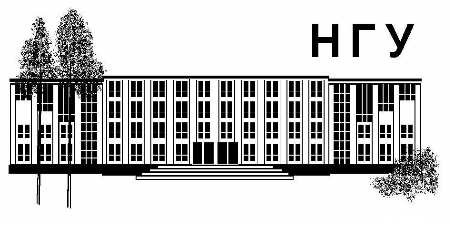
\includegraphics[width=\textwidth]{../NSU-logo}
    \end{minipage}
    \hfill
    \hspace*{6em}

    Кафедра теоретической физики физического факультета НГУ
    \medskip

    \Large
    Профессор Грабовский А.\,В.
    \smallskip

    \huge
    \textbf{Общая теория относительности}
    \smallskip

    \Large
    Семинар № 2
    \vfill

    \normalsize
    \begin{minipage}{0.85\linewidth}
      Вычисление ковариантной производной от метрики. Получение
      символов Кристоффеля из условия $D_kg_{ij}=0$. Построение
      локально-инерциальной системы в заданной точке. Вывод закона
      преобразования символа Кристоффеля при замене
      координат. Доказательство симметричности символа Кристоффеля по
      нижним индексам при условии существования локально-инерциальной
      системы отсчета.
    \end{minipage}
    \vfill

    \normalsize \ccbysa\hspace{0.5em}  Новосибирск 2022
  \end{center}
\end{titlepage}
\end{document}
